\chapter{Test Journal: GPS Variances Test} \label{app:GPSImprovement}

\textbf{Date: TBA}

\subsubsection*{Purpose}
To determine the effectiveness of including base corrections when solving GPS location. Additionally the variance of the GPS is found for the case where the GPS is getting RTK corrections with integer solution, as described in \autoref{app:rtk_gps}.

\subsection*{Equipment}
\begin{itemize}
	\item Emlid Reach RTK GPS connected to the base station as described in Appendix \ref{app:rtk_gps}
  \item Water proof container
  \item HTC Desire HD with access to cellular networks
\end{itemize}

\subsubsection*{Theory}
By comparing the mean and variance of a GPS with and without base correction, the theoretical improvement in precision and accuracy by including base corrections can be shown.\\
Ideally the correct position of the GPS should be recorded over 42 hours or more by placing the GPS in single-mode. This way the average will include a lot of different satellite configurations and no potential bias is added by a base.\\
If the found location is assumed to be correct the accuracy of the proceeding tests can be evaluated with respect to this.\\
For practical reasons this was not prioritized in this project. A 5 hour test was instead performed including all three modes in which the GPS can operate. This is a startup process that the GPS goes through before it receives base corrections and eventually finds a fix for the integer solution.\\
From these results the precision, relevant for the control system, is accessed.
%Under optimal circumstances, this test should be preformed by two similar GPS's at the simultaneously, however it was not a possibility, thus two days with similar weather was chosen as test dates instead.

\subsection*{Procedure}
\begin{enumerate}
  \item Set up the Emlid Reach to log its position in NMEA-format.
	\item Turn on Hotspot on the phone (this should be known to the Emlid Reach module).
	\item Through the reach view app connect the Emlid Reach to the base station.
	\item Put the GPS and Phone in the container.
	\item Place the GPS and phone with access to a power outlet and clear sky view.
	\item Wait 5 hours.
	\item Retrieve the setup and extract the data from the logs recorded on the Emlid Reach.
\end{enumerate}

\subsubsection*{Results}

\begin{figure}[H]
  \captionbox
  {
    
    \label{fig:GPS_2DPlot}
  }
  {
    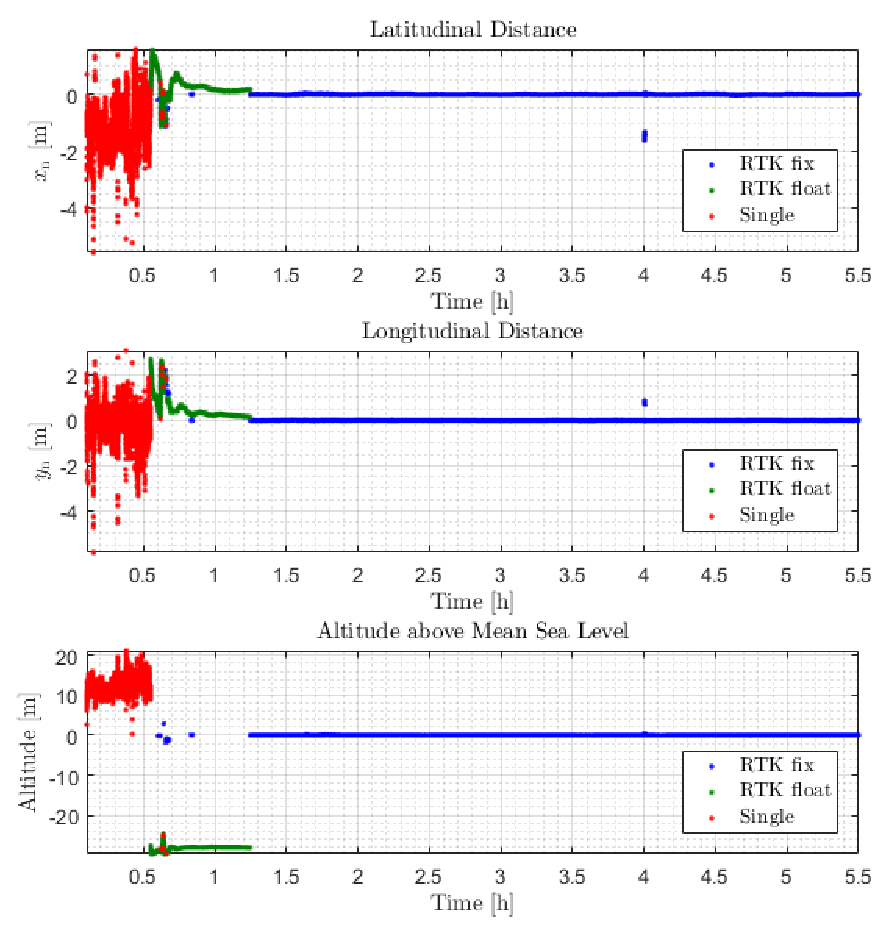
\includegraphics[width=.45\textwidth]{figures/GPS_2DPlot}
  }
  \hspace{5pt}
  \captionbox
  {
    
    \label{fig:GPS_3DPlot}
  }
  {
    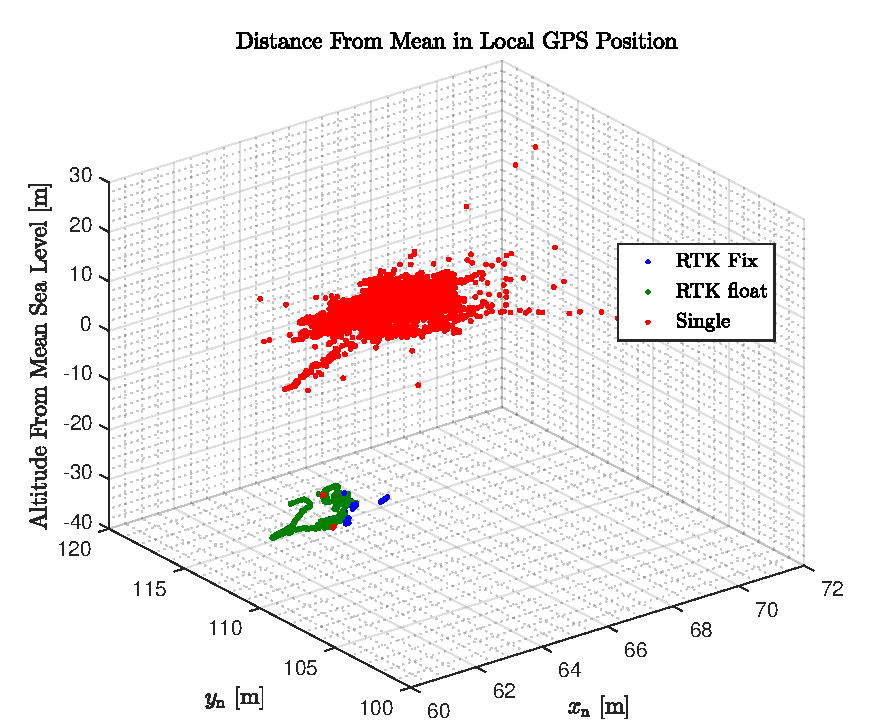
\includegraphics[width=.45\textwidth]{figures/GPS_3DPlot}
  }
\end{figure}

\autoref{fig:GPS_2DPlot}
\autoref{fig:GPS_3DPlot}

\begin{figure}[H]
  \captionbox
  {
    
    \label{fig:GPS_2DPlot_RTK}
  }
  {
    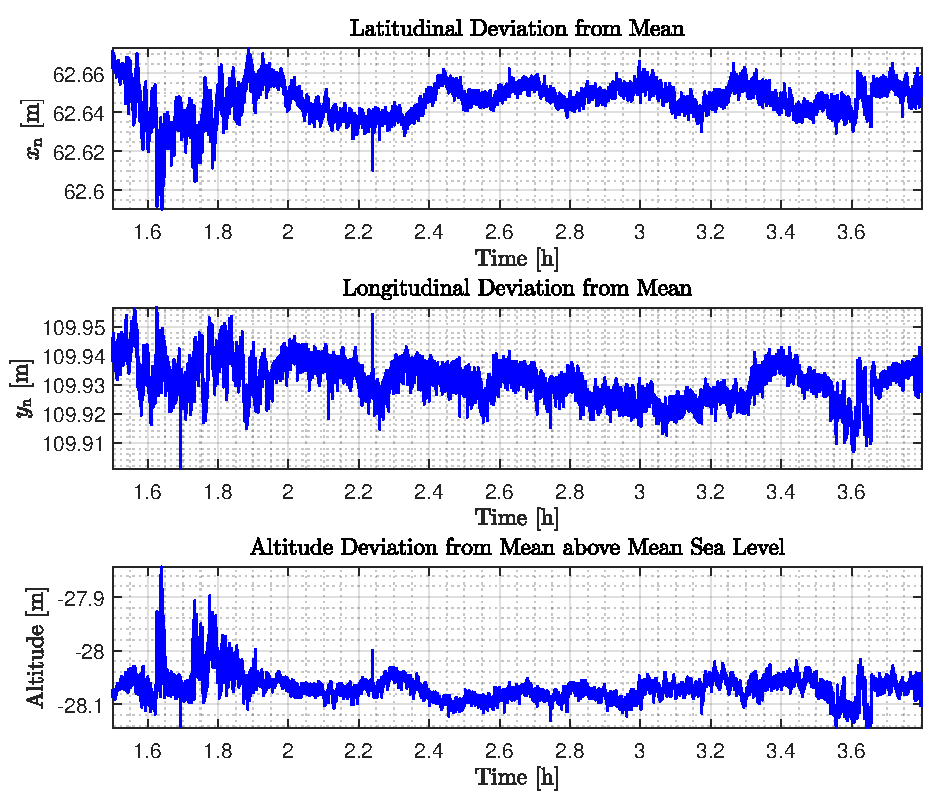
\includegraphics[width=.45\textwidth]{figures/GPS_2DPlot_RTK}
  }
  \hspace{5pt}
  \captionbox
  {
    
    \label{fig:GPS_3DPlot_RTK}
  }
  {
    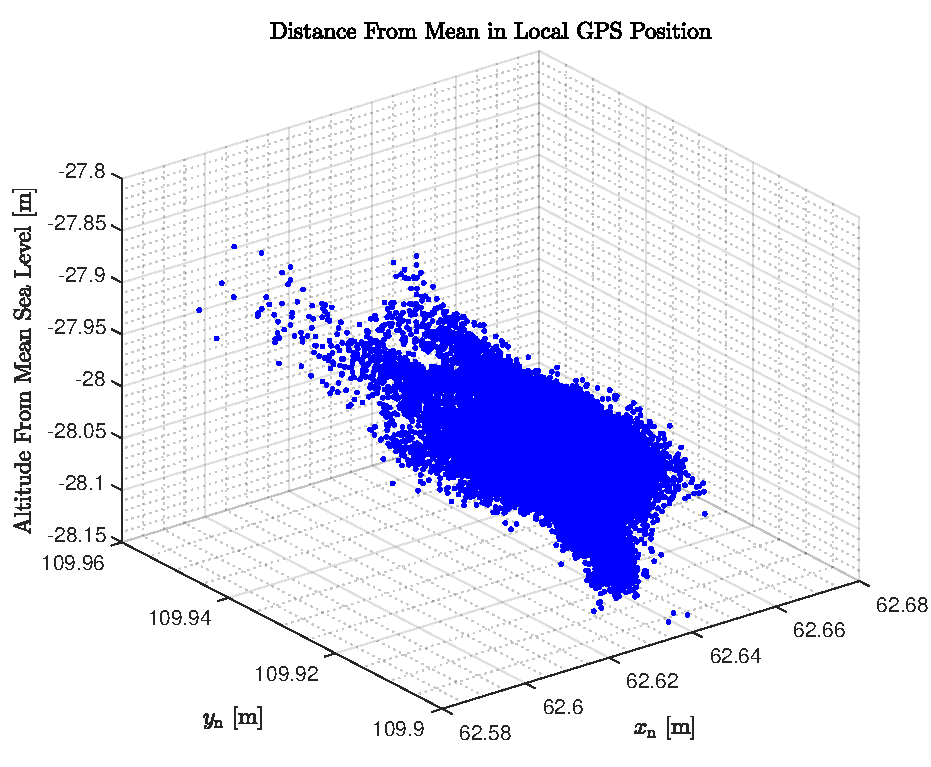
\includegraphics[width=.45\textwidth]{figures/GPS_3DPlot_RTK}
  }
\end{figure}

\autoref{fig:GPS_2DPlot_RTK}
\autoref{fig:GPS_3DPlot_RTK}

\begin{figure}[H]
  \captionbox
  {
    
    \label{fig:GPS_RTK_FIX_Histogram}
  }
  {
    \includegraphics[width=.45\textwidth]{figures/GPS_RTK_FIX_Histogram}
  }
  \hspace{5pt}
  \captionbox
  {
    
    \label{fig:GPS_RTK_FIX_Histogram2}
  }
  {
    \includegraphics[width=.45\textwidth]{figures/GPS_RTK_FIX_Histogram2}
  }
\end{figure}

\autoref{fig:GPS_RTK_FIX_Histogram}
\autoref{fig:GPS_RTK_FIX_Histogram2}


